\documentclass{beamer}
\usepackage[T1]{fontenc}
\usepackage[english]{babel}
\usepackage{amsmath}
\usepackage{graphicx}       
\usepackage{xcolor}         
\usetheme{CVUT} 
\setbeamertemplate{footline}[frame number]
\beamertemplatenavigationsymbolsempty

%%%%% Because of the font Technika, you should use XeLaTex as a comppiler.


%%%%%%% select: CZ, EN
\newcommand{\LANG}{EN}

%%%%%%%% select: light, dark
\newcommand{\FRONTPAGE}{dark}


\title{Presentation Title}
\subtitle{Optional Presentation Subtitle}
\author{Presentation Author}
\institute{Department, Faculty, CTU in Prague}
\date{ABC, 2017}
%%%% set headlines (you can leave it blank)
\newcommand{\headlineA}{CUSTOM HEADLINE}
\newcommand{\headlineB}{HEADLINE B}
\newcommand{\headlineC}{HEADLINE C}


\begin{document}


\begin{frame}
  \clearpage\thispagestyle{empty}\titlepage
\end{frame}

\begin{frame}{Click to add Title}
\begin{itemize}
    \item First
    \item In-line math $a = \sqrt{-1}$
    \item Háčky a čárky se zobrazují v pořádku.
\end{itemize}
\end{frame}

\begin{frame}
    Slide with no slide title. Title or multiple titles can be placed in custom way in body of the slide content.
\end{frame}


\begin{frame}{Latex Equations}
Numbered equation
 \begin{equation}
  L' = {L}{\sqrt{1-\frac{v^2}{c^2}}}
 \end{equation}
Numberless equation
\begin{equation*}
 \lim_{x\to 0}{\frac{e^x-1}{2x}}
 \overset{\left[\frac{0}{0}\right]}{\underset{\mathrm{H}}{=}}
 \lim_{x\to 0}{\frac{e^x}{2}}={\frac{1}{2}}    
\end{equation*}

\end{frame}


\begin{frame}{Example Picture}
    \begin{figure}[]
    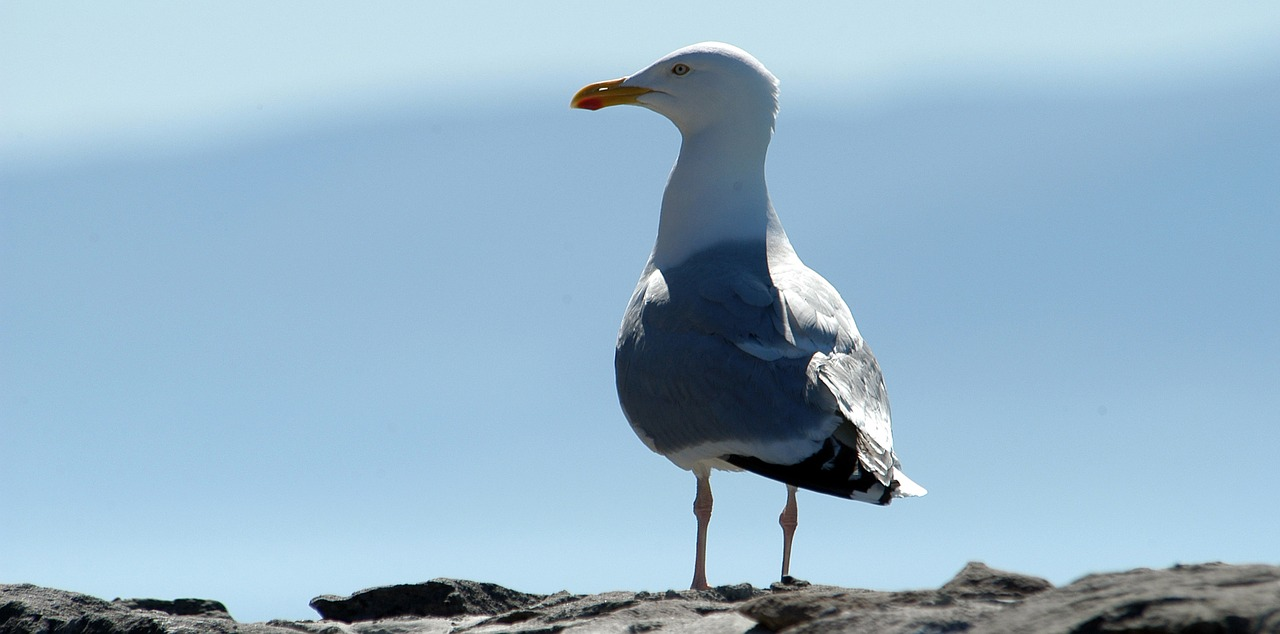
\includegraphics[width=1.\textwidth]{gull.jpg}
    \end{figure}
\end{frame}



\end{document}

